% Template for PLoS
% Version 1.0 January 2009
%
% To compile to pdf, run:
% latex plos.template
% bibtex plos.template
% latex plos.template
% latex plos.template
% dvipdf plos.template

\documentclass[12pt]{article}

% amsmath package, useful for mathematical formulas
\usepackage{amsmath}
% amssymb package, useful for mathematical symbols
\usepackage{amssymb}

% graphicx package, useful for including eps and pdf graphics
% include graphics with the command \includegraphics
\usepackage{graphicx}

% cite package, to clean up citations in the main text. Do not remove.
\usepackage{cite}

\usepackage{color} 
\newcommand{\hilite}[1]{\colorbox{yellow}{#1}}

% Use doublespacing - comment out for single spacing
\usepackage{setspace} 
\doublespacing


% Text layout
\topmargin 0.0cm
\oddsidemargin 0.5cm
\evensidemargin 0.5cm
\textwidth 16cm 
\textheight 21cm

% Bold the 'Figure #' in the caption and separate it with a period
% Captions will be left justified
\usepackage[labelfont=bf,labelsep=period,justification=raggedright]{caption}

% Use the PLoS provided bibtex style
\bibliographystyle{plos2009}

% Remove brackets from numbering in List of References
\makeatletter
\renewcommand{\@biblabel}[1]{\quad#1.}
\makeatother


% Leave date blank
\date{}

\pagestyle{myheadings}
%% ** EDIT HERE **


%% ** EDIT HERE **
%% PLEASE INCLUDE ALL MACROS BELOW

%% END MACROS SECTION

\begin{document}

% Title must be 150 characters or less
\begin{flushleft}
{\Large
\textbf{Title}
}
% Insert Author names, affiliations and corresponding author email.
\\
\author{Alexandra Schnoes$^1$%
       \email{Alexandra Schnoes - alexandra.schnoes@ucsf.edu}%
         David C. Ream$^2$%
         \email{David Ream - reamdc1@miamioh.edu}
      \and
         Alexander Thorman$^2$%
         \email{Alexander Thorman - thormanaaw@muohio.edu}
      \and
         Patricia Babbitt$^1$%
         \email{Patricia Babbitt - babbittp@ucsf.edu}
       \and 
        Iddo Friedberg\correspondingauthor$^{2,3}$%
        \email{Iddo Friedberg\correspondingauthor - i.friedberg@miamioh.edu}
      }
      

%Author1$^{1}$, 
%Author2$^{2}$, 
%Author3$^{3,\ast}$
%% \address{
%%    \iid(1)Department of Bioengineering and Therapeutic Sciences, University of California San Francisco, 
%%            San Francisco, CA, USA\\
%%      \iid(2)Department of Microbiology, Miami University, Oxford, OH USA\\
%%      \iid(3)Department of Computer Science and Software Engineering , Miami University, Oxford, OH USA
%% }%
\bf{1} Author1 Dept/Program/Center, Institution Name, City, State, Country
\\
\bf{2} Author2 Dept/Program/Center, Institution Name, City, State, Country
\\
\bf{3} Author3 Dept/Program/Center, Institution Name, City, State, Country
\\
$\ast$ E-mail: Corresponding author@institute.edu
\end{flushleft}

% Please keep the abstract between 250 and 300 words
\section*{Abstract}

        \paragraph*{Background:} Computational protein function
prediction programs rely upon well-annotated databases for testing and training
their algorithms. These databases, in turn, rely upon the work of curators
to capture experimental findings from scientific literature and apply them to protein
sequence data. However, with the increasing use of high-throughput experimental
assays,  a small number of experimental papers dominate
the functional protein annotations collected in databases. 
Here we investigate just how prevalent is the ``few papers --
many proteins'' phenomenon. We hypothesize that the dominance of high-throughput experiments in
proteins annotation biases our view of the corpus of functions enabled by proteins.
      
        \paragraph*{Results:} We examine the annotation of
UniProtKB by the Gene Ontology Annotation project (GOA), and show that
the distribution of proteins per paper is a log-odd, with 0.06\% of papers
dominating 20\% of the annotations. Since each of the dominant papers
describes the use of an assay that can find only one function or a small
group of functions, this leads to substantial biases, in several aspects, in what we know
about the function of many proteins.

        \paragraph*{Conclusions:} Given the experimental techniques
available, protein function annotation bias due to high-throughput experiments is unavoidable. Knowing
that these biases exist and understanding their characteristics and extent is important for
database curators, developers of function annotation programs, and
anyone who uses protein function annotation data to plan experiments.

% Please keep the Author Summary between 150 and 200 words
% Use first person. PLoS ONE authors please skip this step. 
% Author Summary not valid for PLoS ONE submissions.   
\section*{Author Summary}

\section*{Introduction}

Functional annotation of proteins is a primary challenge in molecular biology
today\cite{Friedberg2006Automated,Erdin2011180,Rentzsch2009210,Fetrow2012}. The ongoing
improvements
in sequencing technology had the emphasis shifting from realizing the \$1000
genome to the 1-hour genome \cite{PMID Stahl2012Toward}. The ability to rapidly and
cheaply sequence genomes is creating a flood of sequence data, which require extensive
analysis and characterization before they can be useful. A large proportion of this work
involves assigning biological function to these newly determined gene sequences, a process
that is both complex and costly \cite{Sboner2011Real}. Furthermore,  the ability to
accurately assign function through computational means is challenging and open problem
\cite{Schnoes2009Annotation}. To aid current annotation procedures and improve computational
function prediction algorithms, sources of high-quality, experimentally derived functional
data are necessary.  Currently, one of the few repositories of such data is the UniProt-GOA
database \cite{Dimmer2012UniProtGO}, which contains both computationally derived and
literature derived functional information. The literature derived information is extracted
by human curators who capture functional data from publications, assign the data to its
appropriate place in the Gene Ontology hierarchy \cite{Ashburner2000Gene} and label them
with appropriate functional evidence codes. The UniProt-GOA database is one of only a small
number of databases that explicitly connects functional data, publication references and
evidence codes to specific, experimentally studied sequences.  In addition, annotations
captured in UniProt-GOA directly impact the annotations in the UniProt/Swiss-Prot database,
widely considered to be a gold standard set of functional annotation
\cite{Schnoes2009Annotation}. 

It is important, therefore, to understand any trends and biases that are
encapsulated by the UniProt-GOA database, as those impact well-used sister
databases and therefore a large number of users worldwide. Furthermore,
any biases would impact function prediction algorithms development and training.

One concern surrounding the capture of functional data from papers is the propensity for
high-throughput experimental work to become a large fraction of the data in UniProt-GOA,
thus having few experiments dominate the protein function landscape. In this work we
analyzed the relative contribution of papers to the experimental annotations in UniProt-GOA.
We found some striking biases, stemming from the fact that a small fraction of papers that
describe high-throughput experiments, disproportionately contribute to the pool of
experimental annotations of model organisms. Consequently, we show that: 1) annotations
coming from high-throughput experiments are mostly less informative than those provided by
low-throughput experiments;  2) annotations from high throughput experiments bias the
annotations towards a limited number of functions, and, 3) many high-throughput experiments
overlap in the proteins they annotate, and in the annotations assigned. Taken together, our
findings offer a comprehensive picture of how the current protein function landscape is
generated. Furthermore, due to the biases inherent in the current system of sequence
annotations, this study serves as a caution to the producers and consumers of biological data
from high-throughput experiments. 


% Results and Discussion can be combined.
\section*{Results}

\subsection*{Articles and Proteins} With the advent of high-throughput experiments it has
become possible to conduct large-scale studies of protein functions.  Consequently, some
studies reveal very specific functional aspects of a large amount of proteins as a result of
the particular type of assay or assays used. To understand the impact of large-scale studies
on the corpus of experimentally annotated proteins, we looked at the UniprotKB Gene Ontology
(GO) annotation files, or UniProt-GOA. UniProt-GOA proteins are individually annotated by one or
more GO terms using a procedure described in \cite{Dimmer2012UniProtGO}. Briefly, this
procedure consists of six steps which include sequence curation, sequence motif analyses,
literature-based curation, reciprocal BLAST\cite{Altschul1997Gapped} searches, attribution
of all resources leading to the included findings, and quality assurance. If the annotation
source is a research article, the attribution includes its PubMed ID. For each GO term
associated with a protein, there is also an \textit{evidence code} which is used to explain
how the association between the protein and the GO term was made.  Experimental evidence
codes include such terms as: Inferred by Direct Assay (IDA) which indicates that ``a direct
assay was carried out to determine the function, process, or component indicated by the GO
term'' or Inferred from Physical Interaction (IPI) which ``Covers physical interactions
between the gene product of interest and another molecule.'' (Taken from the GO site,
geneontology.org).  Computational evidence codes include terms such as \textit{Inferred from
Sequence or Structural Similarity} (ISS) and \textit{Inferred from Sequence Orthology}
(ISO).  However, these are still assigned by a curator. There are also non-computational and
non-experimental evidence codes, the most prevalent being \textit{Inferred from Electronic
Annotation} (IEA) which is ``used for annotations that depend directly on computation or
automated transfer of annotations from a database''. IEA evidence means that the annotation
was not made or checked by a person.  Different degrees of reliability are associated with
the evidence codes, with experimental codes generally considered to be of higher reliability
than non-experimental codes. However, the increase in the number of high-throughput
experiments used to determine protein functions may introduce biases into experimental protein
annotations, due to the inherent capabilities and limitations of high-throughput assays.  

To test the hypothesis that such biases exist, and to study their extent if they
do, we compiled the details of all experimentally-annotated
proteins in UniProtKB. This included all proteins whose GO annotations have
the GO experimental evidence codes EXP, IDA, IPI, IMP, IGI, IEP. We first examined
the distribution of articles by the number of proteins they annotate. The results
are shown in Figure~\ref{fig:papers-prots}. 

As can be seen in Figure\ref{fig:papers-prots}, the distribution of the number of proteins
annotated per paper follows a power-law distribution, $f(x)=a\dot x^k$. 
Using the goodness-of-fit based
method we found a significant fit to $a=7; k=2.59$. 
We therefore conclude that there is indeed a substantial bias in
experimental annotations, in which there are few papers that annotate a large
number of proteins.

To better understand the consequences of such a distribution, we divided the annotating articles
into four cohorts, based on the number of proteins each article annotates.
\textit{Single-throughput} papers are those papers that annotate only one protein; \textit{low
throughput} papers annotate 2-9 proteins; \textit{moderate throughput} papers annotate 10-99
proteins and \textit{high throughput} papers annotate over 99 proteins. The results are shown in
Table~\ref{tab:cohorts}. The most striking finding is that high throughput papers are responsible
for 25\% of the annotations in Uniprot-GOA, even though they comprise 0.08\% of the papers. 96\%
of the papers are single-throughput and low throughput, however those annotate only 53\% of the
proteins in Uniprot-GOA. So while moderate throughput and high-throughput experiments account for
almost half of the annotations in Uniprot-GOA, they comprise only 4\% of the experiments
published.

What typifies high-throughput papers? Also, how may the log-odds distribution bias what we
understand of the protein function universe? To answer these questions, we examined
different aspects of the annotations in the four paper cohorts. Also, we examined in higher
detail the top 50 annotating papers. (Overall, 62 papers in our study annotated more than
100 proteins). 

An initial characterization of the top 50 high-throughput papers is shown in
Table\ref{table:top-papers}.  As can be seen, almost all of the papers are specific to a
single species (typically a model organism) and assay that is used to annotate the proteins
in that organism.  Since a single assay was used, then typically only one ontology (MFO, BPO
or CCO) was used for annotation. For some species this means that a single functional aspect
(MFO, BPO or CCO) of a species will be dominated by a single experiment.

\subsection*{Term frequency bias}

To see how much a single species-- and method-- specific high-throughput assay affects the entire
annotation of a species, we examined the relative contribution of the top-50 papers to the
entire corpus of experimentally annotated protein in each species.  All the species we
examined were model organisms or human, as all the top annotation-contributing papers dealt with model
organisms. For each species, we looked at the five most frequent terms in the top 50
annotating papers. We then examined the contribution of this term by the top 50 papers to the
general annotations of that species.  The \textit{contribution} is the number of annotations
by any given GO term in the top 50 papers divided by the number of annotations by that GO
term in all of UniProtKB.  For example, as seen in Figure~\ref{fig:rel-contrib} in \textit{D.
melanogaster} 88\% of the usage of ``precatalytic splicosome'' is contributed by the top-50
papers. 

% "Annotation Trends" in Alex's poster

For most organisms in the top-50 papers,  the annotations were within the cellular component
ontology. The exceptions are \textit{D. melanogaster} and \textit{C. elegans} where the
dominant terms were from the Biological Process ontology, and in mouse, where ``protein
binding'' and ``identical protein binding'' are from the Molecular Function Ontology.
\textit{D. melanogaster}'s annotation for the top terms is dominated (over 50\% contribution)
by the top-50 papers. 

The term frequency bias described here can be viewed more broadly within the ontology bias. The proteins
annotated by single-protein papers, low-throughput papers, and moderate throughput papers 
have similar ratios of the fraction of proteins annotated.  Twenty-two to twenty-six percent of assigned
terms are in the Molecular Function Ontology, and 51-57\% are in the Biological Process Ontology and the
remaining 17-25\% are in the Cellular Component ontology. This ratio changes dramatically with
high-throughput papers (over 99 terms per paper). In the high-throughput papers, only 5\% of assigned
terms are in the Molecular Function Ontology, 38\% in the Biological Process Ontology and 57\% in the
Cellular Compartment Ontology, ostensibly due to a lack of high-throughput assays that can be used for
generating annotations using the Molecular Function Ontology. 

% The next paragraph should be should be moved to Methods. We'll just write that we removed the
% propagation bias. This is not a finding, it's a technical clean-up.
% EDIT EDIT: probably can do without this finding.
%Another type of annotation bias may result due to GO-structure derived redundancy: the annotation of
%a single term using a given GO-term and one or more of its parents. However, this type of
%annotation may not necessarily be wholly redundant. For example, a protein may localize to
%the nucleolus and the nucleus itself. In the Cellular Compartment ontology, ``nucleus'' is
%a parent term for ``nucleolus''. In the case of this hypothetical protein, annotating with
%``nucleolus'' and ``nucleus'' is not an error. However, if the protein was found to
%localize to the nucleolus only, then annotating with both terms is a redundancy. We termed
%such a redundancy \textit{propagation bias}. We examined all proteins for possible propagation
%bias. If a protein was annotated with a GO term and one or more parent terms, the parent
%terms were removed. We found possible propagation biases in 17 of the 50 papers. The results
%are summarized in Table\ref{tab:prop-bias}. 

\subsection*{Reannotation Bias}

% Text for dream-catcher plots
Another type of annotation bias is that of protein re-annotation. How many of the top-50 papers
actually re-annotate the same set of proteins? And how much of an agreement is there between different
experiments?
To investigate the extent of repetitive annotations in different papers, we clustered all the
proteins annotated by the top-50 papers using CD-HIT\cite{CD_HIT} at 100\% sequence identity. We
then examined the number of clusters containing 100\% identical sequences per model species. The
product of the number of proteins divided by the number of clusters is the redundancy
percentage. For example, if each of the top-50 papers annotating the proteins in a given species
annotated the same protein set, the redundancy percentage would be 100\%. The results of
confirmation bias analysis are shown in Figure~\ref{fig:dreamcatcher1} and in
Table~\ref{tab:dreamcatcher1}. As can be seen, the highest percent redundancy is among the ZZZ
papers annotating {\em C. elegans}. 

(Insert DreamCatcher Figure \& Table Here )

We have determined, therefore, that there is a degree of repetition between experiments in
the proteins they annotate, with some overlaps being quite high. However, there is still the
need to determine the extent of the repetition of the annotation. We therefore analyzed the
100\% sequence identity clusters for overlap in annotation.  To do so, we counted the number
of identical GO-terms per ontology within each cluster, and divided that by the sum of
GO-terms shared between all papers in the cluster. The result is a number between 0 and 1.
Zero means no GO-terms are shared, while one means all GO-terms are shared. 

The results are shown in Figure~\ref{fig:dreamcatcher2} and in
Table~\ref{tab:dreamcatcher2}. In \textit{S.  cerevisiae}, four papers contribute to the
Cellular Component ontology, by annotating 635 proteins which are common between two or more
of these papers. Among those proteins,  79.6\% of the terms produced are identical.

\subsection*{Quantifying annotation information}

A common assumption holds that while high-throughput experiments do annotate more protein
functions than low-throughput experiments, the former also tend to be more shallow in the
predictions they provide. The information provided, for example, by a large-scale protein
binding assay will only tell us if two proteins are binding, but will not reveal whether
that binding is specific, will not provide an exact $K_{bind}$, will not say under what
conditions binding takes place, or whether there is any enzymatic reaction or
signal-transduction involved. Having on hand data from experiments with different
``thorughputness'' levels,  we set out to investigate whether there is a difference in the
information provided by high-throughput experiments vs. low-throughput ones. To answer this
question, we first have to quantify the information given by GO terms. One way to do so, is
to use the depth of the term in the ontology: the term ``enzyme activity'' would be less
informative than ``dehalogenase'' and the latter will be less informative than ``haloalkane
dehalogenase''.  We therefore counted edges from the ontology root term to the GO-term to
determine term information. The larger the number of edges, the more specific -- and
therefore informative -- the annotation. In cases where several paths lead from the root to
the examined GO-term, we used the minimal path. We did so for all the annotating papers
split into groups by the number of proteins each paper annotates. 


Edge counting provides a measure of term-specificity. It is, however, imperfect. The reason is
that different areas of the GO DAG have different connectivities, and terms may have different
depths unrelated to the intuitive specificity of a term. For example ``high-affinity Tryptophan
transporter'', (GO:0005300) is 14 terms deep, while ``anticoagulant'', (GO:0008435) is only three
terms deep.  For this reason, information content, the logarithm of the inverse of the GO term
frequency in the corpus is generally accepted as a measure of GO-term information
content\cite{lord-semsim}. To account for the possible bias created by the GO-DAG structure, we
also used the log-frequency of the terms in the experimentally annotated proteins in Uniprot-GOA.
However, it should be noted that the log-frequency measure is also imperfect because, as we see
throughout this study, a GO-term's frequency may be heavily influenced  by the top annotating
papers, injecting a circularity problem into the use of this metric. Since no
single metric for measuring the information conveyed by a GO term is wholly satisfactory, we used
both in this study.

The results of both analyses are shown in Figure~\ref{fig:go-depth} and the accompanying
Table~\ref{tab:go-depth}. In general, the results from the depth-based analysis and the
log-frequency based analysis are in agreement, when compared across groupings based on the
number of proteins annotated by the papers. For the Molecular Function ontology, the
distribution of edge counts and log-frequency scores decreases as the number of annotated
proteins per-paper increases.  For the Biological Process ontology, the decrease is
significant. However the contributer to the decrease are the high-throughput papers
while there is little change in the first three paper cohorts.
Finally, there is no significant trend of GO-depth decrease in the Cellular Component
Ontology. However, using the information content metric, there is also a significant decrease
in information content in the high-throughput paper cohort.

\subsection*{Annotation consistency}
Another interesting question was how consistent were the annotations between different experiments?


\subsection*{Evidence and Assertion}

There are two complementary ways by which we come to knowledge about a protein's function. The
approximately 20 GO evidence codes, discussed above, encapsulate the type results by which the
function was inferred, but they do not capture all the necessary information. For example,
``Inferred by Direct Assay (IDA)'' informs that experimental evidence was used, but does not say
which type of experiment was performed. This information is often needed for several reasons.
Knowing which experiments were performed can help the researcher establish the reliability and
scope of the data. For example, RNA for RNAi experiment does not traverse the
blood-brain-barrier, meaning that no data from the central nervous system can be drawn from an
RNAi experiment. The Evidence Code Ontology, or ECO, seeks to improve upon the GO-attached
evidence codes. ECO provides more elaborate terms than ``Inferred by Direct Assay'': ECO also
conveys which assay was used, i.e.  ``microscopy''.  In addition to evidence terms, the ECO
ontology provides \textit{assertion terms} in in which the nature of the assay is given. For
example, an enzyme-linked immunosorbent assay (ELISA) provides quantitative protein data
\textit{in vitro} while an immunogold assay may provide the same information, and cellular
localization information \textit{in vivo}. It is therefore important to know both the assertion
and the evidence to understand what sort of information may be gleaned from the assay.  However,
to understand which types of assertions are made in the top-50 high throughput papers, we
performed manually assigned Evidence Codes Ontology (ECO) assertion and evidence terms to the
top-50 papers. The ECO ontology is more elaborate than the evidence codes used by Uniprot-GOA
now. Although there are plans to insert ECO terms into Uniprot GOA in the near future, those will
probably not be done manually for proteins already existing in Uniprot-GOA, but by automatic
mapping EC terms to ECO ontology terms using a preset table (Rachael Huntley, Chris Mungall  and
Tony Sawford, personal communication). Thus, the ECO-based annotations we provide here to the top
50 papers is probably more informative than a future annotation may provide.

The results are shown in Figure~\ref{fig:assertion} and in
Table~\ref{tab:assertion}.

Interestingly, the most frequently used assertion in the top experimental papers was not an
experimental assertion, but rather a computational one: the term ECO:00053 ``computational
combinatorial evidence'' is defined as ``A type of combinatorial analysis where data are
combined and evaluated by an algorithm.'' This is not a computational prediction per-se, but
rather a combination of several experimental lines of evidence used in a paper. 

The most used experimental assertion term was ECO:000160 ``protein separation followed by fragment
identification evidence'', which captures different types of mass-spectrometry experiments.  The
next ranking assertion terms were computational: ``motif similarity evidence'' and ``sequence
similarity evidence used in automatic assertion''.  Those were generally combined with the
mass-spectrometry experiments to identify protein sequence fragments reconstructed from the
mass-spectrometry. Other frequently used experimental techniques used were ``RNAi experimental
evidence''. This type of experiment was mostly with the papers that used RNA interference in
studying \textit{C. elegans}. 

% \subsection*{Annotation quality}
% 
% One reflection on annotation coverage is the number of GO terms assigned to any
% given protein. Ostensibly, the larger the number of GO terms that are assigned to a
% protein, the more comprehensive its annotation, provided that these terms are
% non-redundant, i.e. not direct parents of each other. 
% 
% The median number of annotations per protein was 1.09, which means that most of the top-50
% papers do not provide more than a single GO-term per protein. Also, the mean number of
% annotations per protein was 1.59. The difference between the mean and median reflects that
% most papers have an annotations-per-protein ratio which is close to 1, whereas few have a
% higher annotation ratio. As shown in Figure~\ref{fig:annotation-ratio}, that is essentially
% the case. Seven papers had an annotations per proteins ratio which is above 2. Those
% were paper numbers 1, 4, 10, 23, 34 and 43 on the list. We decided to examine these papers
% to see whether these studies did indeed provide better coverage, and what distinguished them
% from the other high throughput studies. To follow are brief summaries of the
% methodologies used in these papers.
% 
% \textbf{Toward a confocal subcellular atlas of the human proteome.}
% 
% In this microscopy-based study, the authors used specific staining techniques and confocal
% microscopy to describe the subcellular localization of 4937 proteins, which were each assigned
% to one or more of ten different subcellular compartments. Since proteins may be assigned to more
% than a single compartment, there is a mean of 2.23 GO annotations per protein. The most frequent
% terms were ``nucleus'' and ``cytosol'' with 2211 and 2208 terms, respectively. The next
% most frequent terms was``cytoplasm'', ``endoplasmatic reticulum'' and ``golgi apparatus'' with
% 400-500 terms each.  ''\cite{PMID:11121744}. This paper is the top annotating one that we found,
% both in GO-terms per protein, and in total number of proteins annotated. 
% 
% \textbf{RNAi-based studies of \textit{C. elegans}}
% 
% In \cite{PMID:17417969} the authors fed various bacterial clones expressing dsRNA to \textit{C.
% elegans} mutants that are hypersensitive to dsRNA interference. As  a result, they discovered
% novel loss-of-function phenotypes for 393 \textit{C. elegans} genes. In total they reported 5918
% annotations for 1791 proteins.  The functions reported herefact, ere for the Biological Process
% Ontology. Figure 2B 
% 
% The three other studies were also RNAi-based using \textit{C. elegans}. 


\section*{Discussion}

We have identified several annotation biases in UniProt-GOA. These biases stem from the
uneven number of annotations produced by different types of experiments. It is clear that
results from high-throughput experiments contribute substantially to the function annotation
landscape, as up to 20\% of experimentally annotated proteins are annotated by
high-throughput assays, with most of them not being annotated by medium-- or
low--\~throughput experiments. 

At the same time, high throughput experiments produce less information per protein than
moderate--, low-- and single--\~throughput experiments as evidenced by the type of terms
produced in the Molecular Function and Biological Process ontologies. Furthermore, the
number of total GO terms used in the high-throughput experiments is much lower than that
used in low and medium throughput experiments. Therefore, while high throughput experiments
provide a high coverage of protein function space, it is the low throughput
experiments that provide more specific information, as well as a larger diversity of terms.

We have also identified several types of biases that are contributed by high throughput experiments.
First, there is the enrichment of low-information content GO-terms, which means that our
understanding of the protein function as provided by high throughput experiments is limited.
Second, there is the small number of terms used, when considering the large number of proteins that
are being annotated. Third is the general term bias towards the cellular component ontology and, to
a lesser extent, the Biological Process ontology; at the same time, there are very few papers that
deal with the Molecular Function ontology.  These biases all stem from a single source, the inherent
capabilities and limitations of the hight-throughput experiments. 

The most frequent experiment performed is cell fractionation and mass-spectrometry to assign a
Cellular Component ontology terms (citations).  Consequently this means that the assignment
procedure is limited to the cellular compartments that can be identified with the fractionation
methods used\cite{MS-papers}. So while Cellular Component is the most frequent annotation used,
mass-spectrometry is the most common method to localize proteins in components. A notable exception
to the use of MS for protein localization is in the top annotating paper \cite{18029348} which uses
microscopy for subcellular localization. The only MS experiment in the top-50 papers 
whose proteins were not annotated with cellular localization was ``Proteome survey reveals
modularity of the yeast cell machinery''\cite{18029348}. The resulting annotation was ``protein
binding'' form the Molecular Function ontology. A more detailed discussion on this study follows in
the section \textbf{Information Capture} below.

The second most frequent type of experiments used RNA Interference (RNAi) whole-genome gene
knockdowns in \textit{C. elegans}, \textit{D. melanogaster} and one in \textit{C. albicans}.  RNAi
experiments typically use targeted dsRNA which is delivered to the organism and silences specific
genes. Typically the experiments here used libraries of RNAi targeted to the whole exome. The
phenotypes searched for were mostly associated with embryonic and post-embryonic development
\cite{relevant papers}. Some studies focused on mitotic spindle assembly\cite{17412918}, lipid
storage\cite{17412918} and endocytic traffic\cite{17412918}. One study used RNAi and MP to identify
mitochondrial protein localization \cite{18433294}.

These two types of assays (mass-spectrometry and RNAi)  were strongly linked to the other
frequently used experimental ECO terms, by the nature of the methodology used. Thus, ``protein
separation followed by fragment identification evidence'' is usually accompanied with ``cell
fractionation evidence'' and ``Western blot evidence''. ``RNAi experimental evidence'' is
generally associated with ``mutant phenotype evidence used in manual assertion''. All experiments
are associated with computational ECO terms, which describe sequence similarity and motif
recognition techniques used to identify the sequences found. Thus, a strong reliance on
computational annotation is an integral part of high throughput experiments. It should be noted
that computational annotation here is not necessarily used for functional annotation, but rather
for identifying the protein by a sequence or motif similarity search.

\subsection*{Information Capture and Scope of GO}

So far we have discussed the information loss that is characteristic of high-throughput
experiments, due to the nature of these experiments. However, another reason for information loss
is the inability to capture information using the Gene Ontology. GO is knowingly limited to three
aspects (MF, BP and CC) of biological function, which are assigned per protein. However, other
aspects of function may emerge from 
Of note
is the study mentioned earlier, ``Proteome survey reveals modularity of the yeast cell
machinery''\cite{18029348}.  In this study, the information produced was primarily of protein
complexes and the only GO-term captured in the curation was ``protein binding''.  However, the
study does provide more information than simply which proteins bind others, as  a lengthy catalog
of specific binding partners. Some, but not all of this information can be captured by the
children of the term ``protein binding''. Such a process is arguably laborious by manual
curation. Furthermore, the main information conveyed by this paper, namely the types of protein
complexes discovered and how they relate to cellular networks, is outside the scope of GO. It is
important to realize that while high-throughput experiments do convey less information per
protein within the functional scope as defined by GO, they still convey other, valuable
information which needs to be captured into annotation databases by means other than GO. In the
example above, the information can be captured by a protein interaction database, but not by GO
annotation.

\section*{Conclusions}

Taken together, the annotation biases noted in this study affect our understanding of protein
function space. This, in turn, affects out ability to properly understand the connection between
predictors of protein function and the actual function -- the hallmark of computational function
annotation. As a dramatic example, during the Critical Assessment of Function Annotation
experiment (Radivojac \textit{et al} in review) we have noticed that about 20\% of the proteins
participating in the challenge were annotated as ``protein binding''. This particular This
GO-term is not an informative one. Furthermore, it was shown that the major contribution of this
term  to the CAFA challenge data set was due to high-throughput assays. (Over 100 annotated
proteins annotated per experiment). The concentration of a large number of annotations in a small
number of studies provides only a partial picture of the function of these proteins. As we have
seen, the picture provided is mainly of: 1. subcellular localization cell fractionation and MS
based localization and 2. developmental phenotypes. While these data are important, we should be
mindful of this bias when examining protein function in the database, even those annotations
deemed to be of high quality, i.e. with experimental verification. Furthermore, such a large
bias in prior probabilities is can adversely affect programs employing prior probabilities in
their algorithms, as most machine-learning programs do. Many researchers use programs based on
machine learning algorithm to predict the function of unknown proteins. If the training set for
these programs has included a disproportional number of annotations by thigh-throughput
experiments, the results these programs provide will be strongly biased towards a few frequent and
shallow GO-terms.

Several steps can be taken to remedy this situation. Annotations are derived from
high-throughput experiments can be flagged as such in the database. The flagging can then be
read by sequence similarity or other search software, and flagged proteins removed or
otherwise tagged in the search.  In a typical scenario, a researcher will BLAST their query
protein to determine its function by sequence similarity. If a target protein is tagged as
annotated by a high throughput assay, it would be removed form the search if asked to do so
by the user. This filtering can also be done by assay type, number of proteins annotated per
experiment, or a combination of the above. This requires that GO-annotated proteins should
also be annotated with assertion codes in addition to the evidence codes and GO term-codes;
but given the large volume of data in UniprotKB is it hard to expect such massive
reannotation with assertion terms undertaken. \hilite{(Any other ideas?)}



% You may title this section "Methods" or "Models". 
% "Models" is not a valid title for PLoS ONE authors. However, PLoS ONE
% authors may use "Analysis" 
\section*{Materials and Methods}
We used the Uniprot-GOA database from December 2011. Data analyses were performed using Python scripts.
ECO terms classifying the proteins in the top 50 experiments were assigned to the proteins
manually after reading the articles. All data and scripts are available on
http://github.com/FriedbergLab

% Do NOT remove this, even if you are not including acknowledgments
\section*{Acknowledgments}
We thank Predrag Radivojac, members of the Friedberg and Babbitt labs for insightful discussions.
This research was funded, in part by NSF / ABI XXXXXXX-XXX award to IF and XXXXXXXXXXXX to PCB.

\section*{References}
% The bibtex filename
\bibliography{sp_bias.bib}

\section*{Figure Legends}
%\begin{figure}[!ht]
%\begin{center}
%%\includegraphics[width=4in]{figure_name.2.eps}
%\end{center}
%\caption{
%{\bf Bold the first sentence.}  Rest of figure 2  caption.  Caption 
%should be left justified, as specified by the options to the caption 
%package.
%}
%\label{Figure_label}
%\end{figure}

\begin{figure}[!ht]
\begin{center}
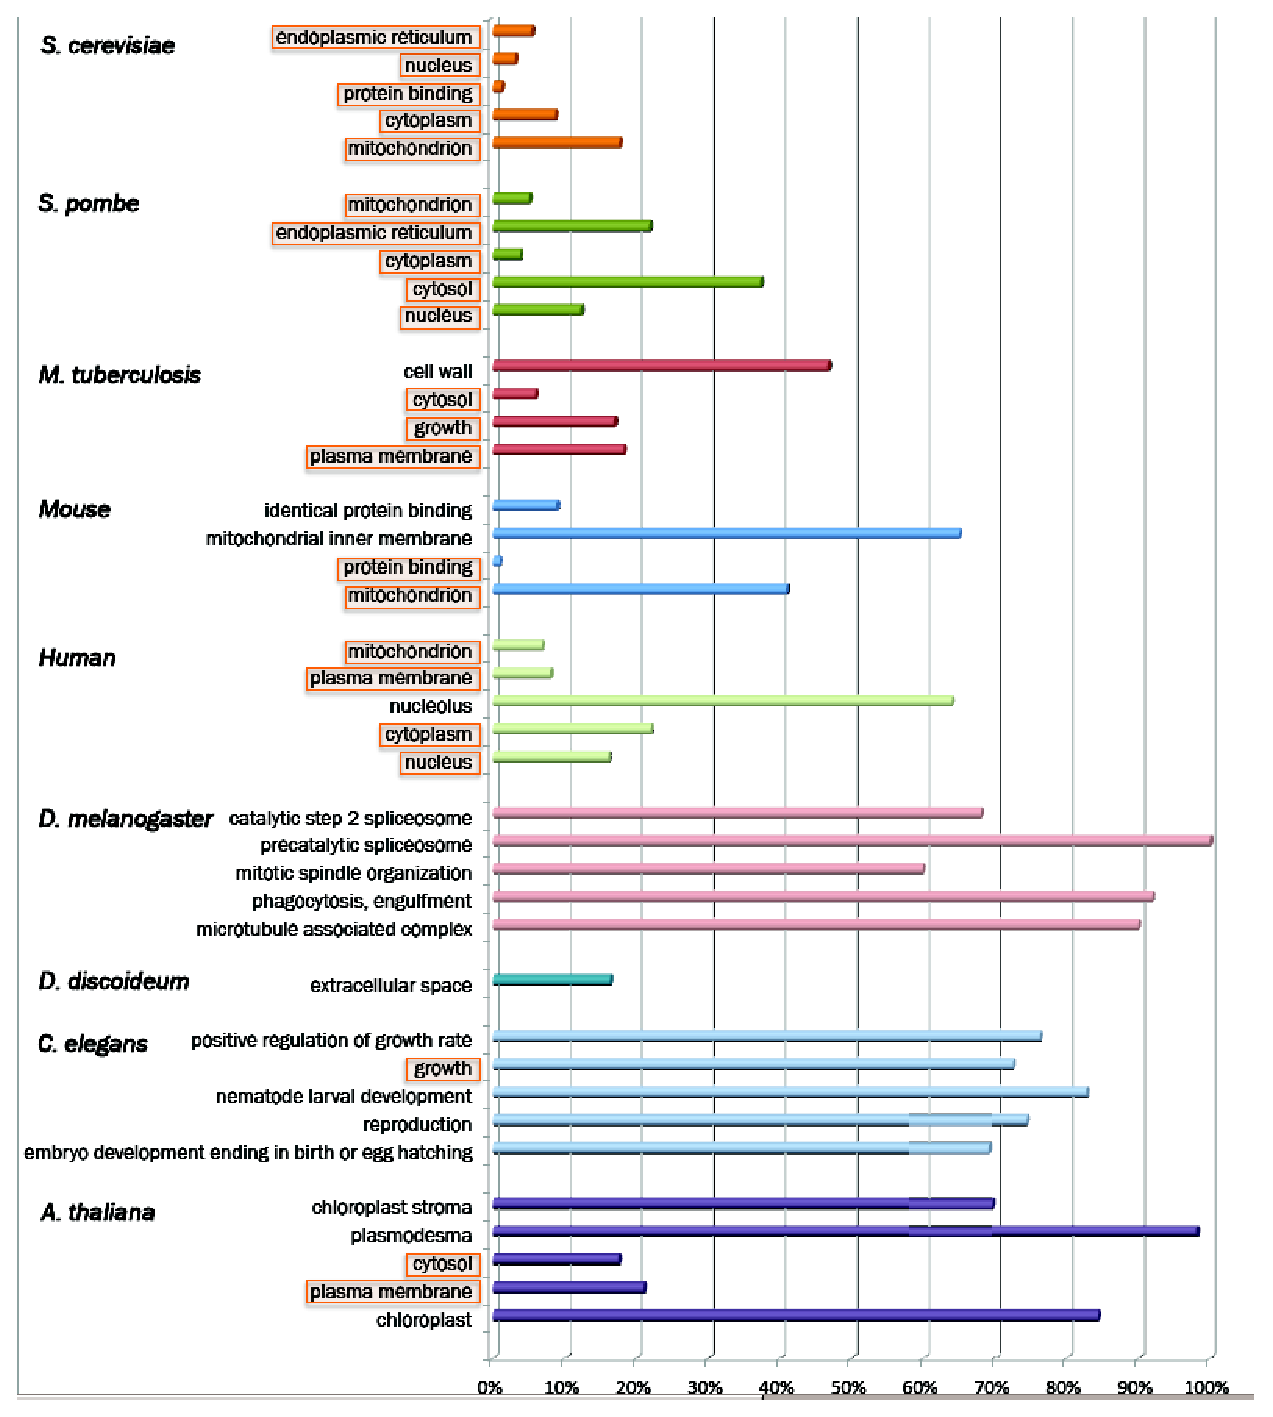
\includegraphics[width=6in]{rel-contrib.eps}
\end{center}
\caption{
{\bf Bold the first sentence.}  Rest of figure 2  caption.  Caption 
should be left justified, as specified by the options to the caption 
package.
}
\label{fig:rel-contrib}
\end{figure}

\section*{Tables}
%\begin{table}[!ht]
%\caption{
%\bf{Table title}}
%\begin{tabular}{|c|c|c|}
%table information
%\end{tabular}
%\begin{flushleft}Table caption
%\end{flushleft}
%\label{tab:label}
% \end{table}

\begin{table}[!ht]
\caption{
\bf{Annotation Cohorts}}
\begin{tabular}{||p{5cm}||l|l|l|l||l||}
\hline
Papers annotating the following number of proteins & 1 & $2<n<10$ & $10<n<100$ & $n>100$ 
& SUM \\ \hline
Number of proteins annotated & 20699 & 46383 & 26485 & 31411 & 124978 \\ \hline
Number of annotating papers & 41156 & 32201 & 2668 & 62 &  76087 \\ \hline
Percent of proteins annotated & 16.56 & 37.11 & 21.19 & 25.13 & 100 \\ \hline
Percent of annotating papers & 54.09 & 42.32 & 3.51 & 0.08 & 100 \\ \hline 
\end{tabular}
\begin{flushleft}Table caption
\end{flushleft}
\label{tab:cohorts}
\end{table}

\begin{table}[!ht]
\caption{
\bf{Annotation Consistency in Top 50 papers}}
\begin{tabular}{|p{3cm}|l|l|l|l|l|l|l|}
\hline
Species & Ontology & Nclust & Mean & Stdv & Stderr & Npapers & Nterms \\ \hline
\textit{A. thaliana} & BPO & 0 & 0 & 0 & 0 & 1 & 1 \\ \hline
\textit{A. thaliana} & CCO & 1883 & 0.082 & 0.271 & 0.006 & 15 & 18 \\ \hline
\textit{C. elegans} & BPO & 1847 & 0.127 & 0.258 & 0.006 & 12 & 41 \\ \hline
\textit{C. elegans} & CCO & 0 & 0 & 0 & 0 & 1 & 1 \\ \hline
\textit{D. melanogaster} & BPO & 15 & 0.3 & 0.245 & 0.063 & 3 & 8 \\ \hline
\textit{D. melanogaster} & CCO & 15 & 0 & 0 & 0 & 3 & 5 \\ \hline
\textit{H. sapiens} & MFO & 0 & 0 & 0 & 0 & 1 & 2 \\ \hline
\textit{H. sapiens} & CCO & 83 & 0.325 & 0.36 & 0.04 & 2 & 20 \\ \hline
\textit{M. musculus} & MFO & 0 & 0 & 0 & 0 & 1 & 2 \\ \hline
\textit{M. musculus} & CCO & 800 & 0.672 & 0.469 & 0.017 & 3 & 2 \\ \hline
\textit{S. pombe} & BPO & 0 & 0 & 0 & 0 & 1 & 4 \\ \hline
\textit{S. pombe} & CCO & 0 & 0 & 0 & 0 & 1 & 12 \\ \hline
\textit{S. cerevisiae} & MFO & 0 & 0 & 0 & 0 & 1 & 1\\ \hline
\textit{S. cerevisiae} & CCO & 635 & 0.796 & 0.383 & 0.015 & 4 & 15\\ \hline
\textit{B. tuberculosis} & MFO & 0 & 0 & 0 & 0 & 0 & 0\\ \hline
\textit{B. tuberculosis} & BPO & 0 & 0 & 0 & 0 & 1 & 1\\ \hline
\textit{B. tuberculosis} & CCO & 321 & 0.457 & 0.41 & 0.023 & 2 & 3\\ \hline
\end{tabular}
\begin{flushleft}Table caption
\end{flushleft}
\label{tab:dreamcatcher2}
\end{table}

\end{document}
